% Definitions
\newcommand\wtfgenes{WTFgenes}

% Abstract
\structabs{
A common technique for interpreting experimentally-identified lists of genes
is to look for enrichment of genes associated to particular Gene Ontology terms.
The most common technique uses the hypergeometric distribution;
more recently, a model-based approach was proposed.
These approaches must typically be run using downloaded software, or on a server.
}{
We develop a collapsed likelihood for model-based gene set analysis and present \wtfgenes, an implementation of both hypergeometric and model-based
approaches, that can be published as a static
site with computation run in JavaScript on the user's web browser client.
Apart from hosting, zero server resources are required: the site can (for example) be served
directly from an S3 bucket.
A faster C++ implementation yielding identical results is also provided.
Our implementation of model-based Gene Ontology enrichment uses some optimizations
which permit probability parameters to be integrated out directly.
}{
\wtfgenes\ is available from \url{https://github.com/evoldoers/wtfgenes}.
}{
Ian Holmes {\tt ihholmes+wtfgenes@gmail.com}.
}{
None.
}

\section*{Introduction}

Gene Set Enrichment Analysis (GSEA) \cite{pmid16199517}
Numerous implementations e.g. GO::TermFinder \cite{pmid15297299}

Model-based Gene Set Analysis (MGSA) \cite{pmid20172960}
Bioconductor \cite{pmid21561920}

builds on earlier generative model by \cite{pmid18676451}

% description of MGSA from Bauer et al 2010

\begin{figure}
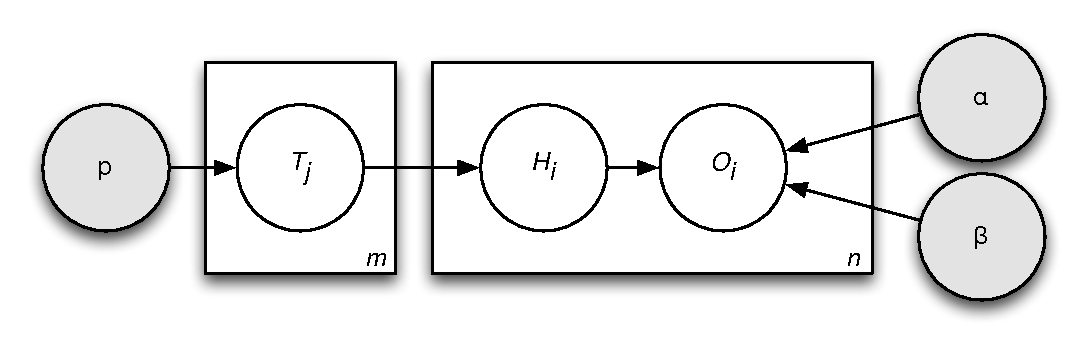
\includegraphics[width=\columnwidth]{model}
\caption{
  \label{fig:model}
  The model
}
\end{figure}

The MGSA model is sketched in Figure~\ref{fig:model}.
For each of the $m$ terms there
is a boolean random variable
$T_j$ (``term $j$ is activated'').
For each of the $n$ genes there is a directly-observed boolean random variable
$O_i$ (``gene $i$ is observed in the gene set''),
and one deterministic boolean variable
$H_i$ (``gene $i$ is activated'')
defined by $H_i = 1 - \prod_{j \in G_i} T_j$
where $G_i$ is the set of terms associated with gene $i$
(including directly annotated terms, as well as ancestral terms implied by transitive closure of the directly annotated terms).
The probability parameters are $\pi$ (term activation), $\alpha$ (false positive) and $\beta$ (false negative),
and the respective hyperparameters are ${\bf p}=(p_0,p_1)$, ${\bf a}=(a_0,a_1)$ and ${\bf b}=(b_0,b_1)$.
The model is
\begin{eqnarray*}
P(T_j=1|\pi) & = & \pi \\
P(O_i=1|H_i=0,\alpha) & = & \alpha \\
P(O_i=1|H_i=1,\beta) & = & 1-\beta
\end{eqnarray*}
with
$\pi \sim \mbox{Beta}({\bf p})$,
$\alpha \sim \mbox{Beta}({\bf a})$ and
$\beta \sim \mbox{Beta}({\bf b})$.
The model of \cite{pmid20172960} is similar but used an
{\em ad hoc} discretized prior for $\pi$, $\alpha$ and $\beta$.

Most MGSA and GSEA implementations are designed for desktop use.

Several GSEA implementations are designed for web use, notably Enrichr \cite{pmid23586463,pmid25971742,pmid27141961}
which has a rich dynamic web front-end.
However these web-facing GSEA implementations generally require a server-hosted back end.
Further, there are no web-based MGSA implementations.

\section*{Results}

We sample from a collapsed version of the model by integrating out the probability parameters.
Let $c_p = \sum_j^m T_j$ count the number of activated terms,
$c_g = \sum_i^n H_i$ the activated genes,
$c_a = \sum_i^n O_i(1-H_i)$ the false positives and
$c_b = \sum_i^n O_i H_i$ the false negatives.
Then
\[
P({\bf T},{\bf O}|{\bf a},{\bf b},{\bf p}) =
Z(c_p;m,{\bf p})
Z(c_a;n-c_g,{\bf a})
Z(c_b;c_g,{\bf b})
\]
where
\[
Z(k;N,{\bf A}) =
\left( \begin{array}{c} N \\ k \end{array} \right)
\frac{B(k+A_0,N-k+A_1)}{B(A_0,A_1)}
\]
is the beta-binomial distribution for $k$ successes in $N$ trials with pseudocounts $(A_0,A_1)$,
using the beta function
\[
B(x,y) = \int_0^1 t^{x-1}(1-t)^{y-1} dt = \frac{\Gamma(x)\Gamma(y)}{\Gamma(x+y)}
\]
Integrating out probability parameters improves sampling efficiency
and allows for future model variations where, for example, we observe multiple gene sets and give each gene its own false positive parameter $\beta_i$.
Our implementation by default uses uninformative priors with hyperparameters ${\bf a}={\bf b}={\bf p}=(1,1)$
but this can be overridden by the user.

For MCMC we use a Metropolis-Hastings sampler where each proposed move perturbs some subset of the term variables.
These moves include {\em flip}, where a single term is toggled;
{\em step}, where any activated term and any one of its unactivated ancestors or descendants are toggled;
{\em jump}, where any activated term and any unactivated term are toggled; and
{\em randomize}, where all term variables are uniformly randomized.
The relative rates of these moves can be set by the user;
after some empirical investigation of mixing efficiency, we set the defaults such that
{\em flip}, {\em step}, and {\em jump} are equiprobable,
while {\em randomize} is disabled.

The non-model based GSEA implementation uses a standard one-tailed Fisher's Exact Test with a Bonferroni correction
for multiple hypothesis testing.

We present JavaScript implementation of MGSA and GSEA, allowing easy comparison.
Static site: can be hosted as static files, inexpensively and with considerable security benefits

For reference we also provide C++ implementation that should yield numerically identical results
(MCMC uses same random number generator)

Autocorrelation plots

Speed comparison: C++ vs JavaScript

\section*{Discussion}

Not a direct competitor to Enrichr, which has much richer visualizations and allows user submission of gene sets

GREAT \cite{pmid20436461}

\section*{Funding}

IHH was partially supported by NHGRI grant R01-HG004483.

\bibliographystyle{natbib}
%\bibliographystyle{bioinformatics}
%\bibliographystyle{achemnat}
%\bibliographystyle{plainnat}
%\bibliographystyle{abbrv}
%
%\bibliographystyle{plain}
%
%\bibliography{Document}


\bibliography{references}
